\section{Coincidence Cave}
    \begin{marginfigure}
        \begin{tikzpicture}
            \node [name-dest] (box){%
                \begin{minipage}{0.80\textwidth}
                    \begin{itemize}
                        \item Rhys Tyers
                        \item Jack Hare
                        \item Jim Evans
                        \item Dave Wilson
                        \item Dewi Lloyd
                        \item Pete Hambley
                        \item Katy Morgan
                    \end{itemize}
                \end{minipage}
            };
            \node[fancytitle, right=10pt] at (box.north west) {Coincidence Cave};
        \end{tikzpicture}
    \end{marginfigure}


    Rhys and James returned to the bivi, buzzing with excitement about the new passage they had found, Jetstream. We entered the survey data into the OLPC, and found that the passage ran due south, towards the face of Mig. We could hardly have been more excited - the prospect of a lower entrance seemed clear, and the glory would clearly go to the ones who found it. With no prospect of going underground, I resolved to search on the surface, and on the next day, put my plan into action.

    I spent some time learning how to use the survey software, and this provided a coordinate for the location directly above the end of Jetstream. It seemed reasonable to begin our search for the lower entrance there. After a great deal of anguish dealing with the conversion between Slovenian coordinates and the more commonly supported UTM, I realised that all I really needed was a bearing and direction from something we already had a UTM coordinate for, namely Gardeners? World. Our torturous calculations are included in the bivi log book. Spookily, the end of Jetstream is absolutely due south of Gardener?s world. I entered the coordinates of our prize into a GPS, and Rhys and I set off above ground to find it.

    The day was ridiculously hot, and we had not brought enough water. We dropped down the east side of Mig towards Gardeners? World. Instead of following Janet?s path to Razor, we decided to cut across a thicket of dwarf pine. I recommend against this route - almost anything is quicker than pushing through dwarf pine, and we became hot, sweaty and dehydrated in no time.

    Eventually, we regained Janet?s path, and followed it round to a junction with several real paths. We took the western route, back towards Kal - we knew we were still too far north, but we weren?t aware of another path, and we decided we could always drop off the path to the south when we got to the right location.

    As we walked, it became clear that the mountain was steeply sloping, and that it would be difficult to actually leave the path to go looking. We continued along, hoping for a break in the trees, and as we arrived at the point due north of our goal, we came across a canyon. This dry canyon runs directly south from the face of Migovec, bisecting the path. It is not very deep, more of a scoured river bed, but it runs down over steep terrain. At the bottom of the canyon we could clearly see Ravne.

    We were hundreds of meters too far north, but the canyon was incredible - Rhys didn?t remember anyone mentioning it before, though it was hardly hidden! We started to down climb it, scrambling over boulders and down short cascades for a few tens of metres. Soon it became too steep, and we worried we wouldn?t be able to climb back up, so we retreated to the path.

    At the point, we recalled a path lower down that followed a parallel path, contouring along the cliff face. It splits off just before the final forest that precedes Kal. So we headed to Kal, stocked up on water and apple sours, and the continued down into the blissful shade. Very soon we refound the canyon, and could see it extend far north to the face of Migovec and far south to Kal. We were very excited, and dumped out light bags to climb up the dry canyon. The free climbing seemed sketchy this first time, and I almost walked into a web with a huge spider waiting to devour me. 

    After checking a few obvious holes, we hit the jackpot around 40 metres up. In a vertical section of the canyon was a dark hole, just body sized, pushing horizontally into the rock. It smelled damp and the air coming out was cold. Sticking my head inside, the size of the draught was obvious. It was clear that this was a strong lead, and Rhys and I were very excited.

    We made our way back to the path, resolving to look south down the canyon before heading back to the bivi to pick up digging supplies. As we drank our water and rested, we heard familiar voices approaching along the path. It was Dave W, Dewi and Pete, this year known as the Three Wise Men. They?d been hunting for the lower entrance for the past two weeks, and had been dragged up a terrible route by Pete?s GPS. We explained what we?d found, and Pete confidently announced that he had already GPS tagged this cave, but that it didn?t go.

    Dewi was unconvinced, and we led him up to the cave. He became immediately excited, screaming insults at Pete and pulling out huge chunks of rock with his bare hands. An impromptu digging party occurred, but without our kit we didn?t make much progress. It did become clear that this was going to be a big job, and no easy break through. After some debate, we agreed to name the lead ?Coincidence Cave? in honour of the great coincidence that occurred. The name that Rhys and I proposed, ?Seren-fucking-dipity Cave? was not considered adequately solemn.

    \begin{figure*}[t!]
        \checkoddpage \ifoddpage \forcerectofloat \else \forceversofloat \fi
        \centering

        \begin{subfigure}{0.644\textwidth}
            \centering
            \frame{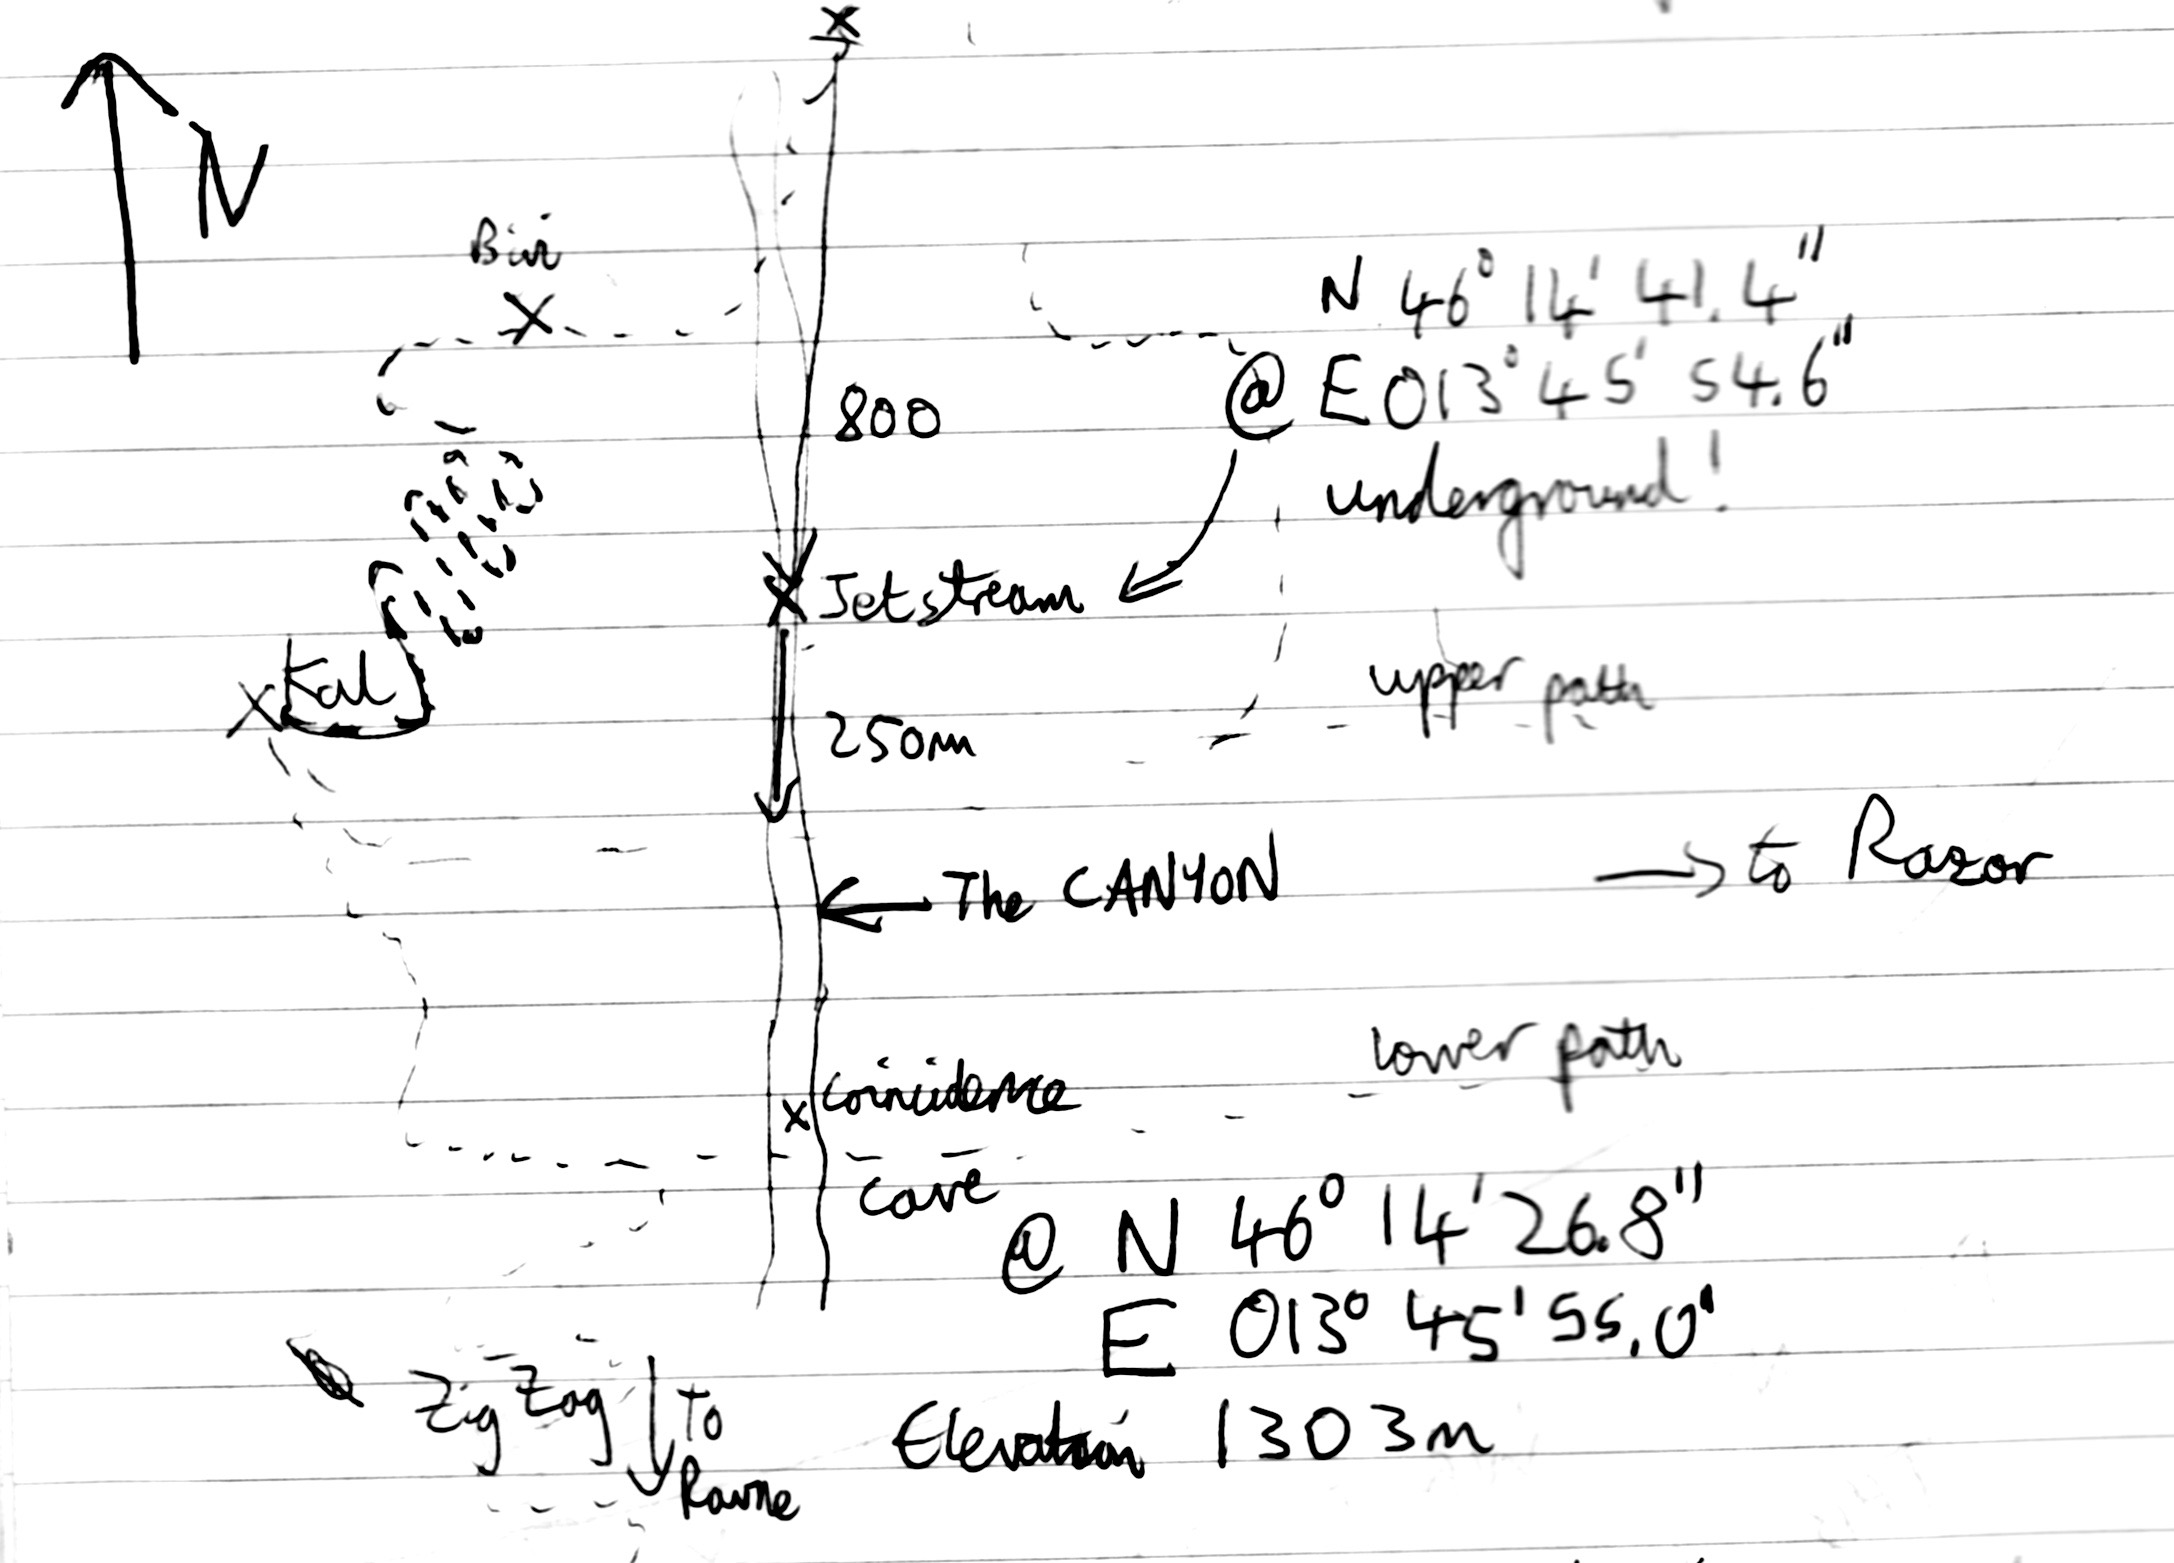
\includegraphics[width=\linewidth]{images/2015/jack-coincidence-2015/migovec_cartoon_5.jpg}}
            \caption{}\label{cartoon}
        \end{subfigure}
        \hfill
        \begin{subfigure}{0.346\textwidth}
            \centering
            \frame{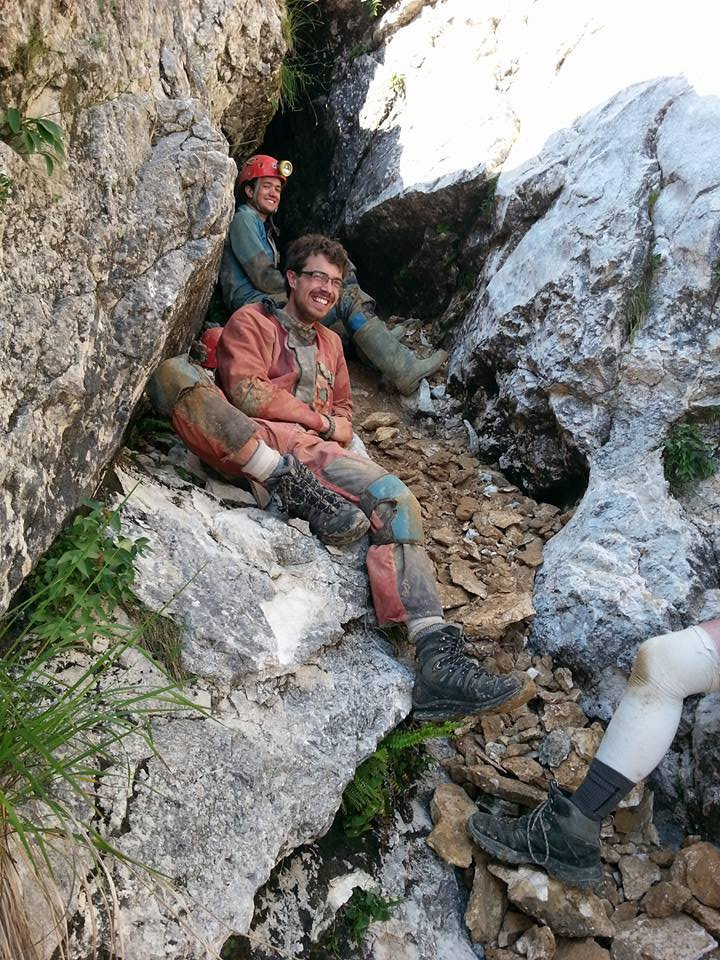
\includegraphics[width=\linewidth]{images/2015/jack-coincidence-2015/jack-coincidence2015.jpg}}
            \caption{}\label{coincidence cave}
        \end{subfigure}

        \caption{
            \emph{(a)} A plan to find the way into the system from the south face of Migovec resulting in the finding of Coincidence Cave --- scanned from 2015 Bivi logbook
            \emph{(b)} After the discovery of Coincidence Cave and a short digging session, elation and disbelief fight it out on the cavers' faces --- Pete Hambly}
        \label{}

    \end{figure*}

    Over the next few days I returned to the dig, commuting from the Bivi with my caving kit. These were long, tiring days, and I joined with Dewi, Dave and Pete in digging shifts of around half an hour. Progress was slow and tedious, but I learned a lot about digging. At the deepest limits of the dig, a loud, low rumbling sound seemed to come from the passage ahead. At first I assumed it was thunder, but when I got out of the dig, I found that there hadn?t been any. This noise would be consistent with a waterfall.

    Jim Evans joined us on one day and showed a great deal of enthusiasm. On my last day on Mig, I waited with Katy Morgan for a smoke signal that Tanguy and Rhys were going to set, but we saw nothing. Later it transpired that they hadn?t set the smoke signal, so that makes sense.

    Further exploration of Jetstream found a passage that extends even further south than Coincidence Cave, and deeper underground. If Coincidence Cave is a lower entrance to the system, as I believe, then it enters into passages at a higher level than those we can push from underground. This alone is enough to tempt me back to the dig.

    \name{Jack Hare}
